\documentclass[../main.tex]{subfiles}
\begin{document}

In this chapter, using researched foundation theories in Chapter~\ref{chapter:literature}, I will present (i) the overview of the AI module as well as an outline of how it is integrated into a larger management system, (ii) the proposed AI module in detail, (iii) hardware implementation, and (iv) the utilization of frameworks.
\section{Overview}
\label{sec:overview}

\begin{figure}[h!]
\centering
\includegraphics[width=\linewidth]{Figure/overview.pdf}
\caption{The overview of a full end-to-end system.}
\label{fig:overview}
\end{figure}

Figure~\ref{fig:overview} shows the overview of a full end-to-end human monitoring system. This system has peripheral devices like cameras to capture frames or sensors to collect environmental parameters. A small, single-board, low-power computer, Jetson Nano is in charge of edge computing, it receives data from sensors and sends them to the server. Furthermore, it takes the stream from the attached camera and conducts all the AI computing tasks, and then sends the processed information to the server to store. Jetson Nano devices are placed at the entrance and in multiple positions inside different rooms to monitor. This system also has a server to store data sent from Jetson Nano and handle requests from user applications. Finally, the end-user application can show statistics and do visualization based on information received from the server.

\begin{figure}[h!]
\centering
\includegraphics[width=\linewidth]{Figure/edge_overview.pdf}
\caption{The overview of the AI module on edge devices.}
\label{fig:edge_overview}
\end{figure}

The scope of this thesis only focuses on the development of the AI module on edge devices as shown in Figure~\ref{fig:edge_overview} and other parts of this system are developed by other members of my research team. Jetson Nano receives input frames captured by the attached camera. Then, the object detection model detects humans on these frames and outputs the corresponding bounding box for each person. Next, the ROI of each person on the image is cut based on the bounding box and fed to the feature extraction model. This model takes images as input and extracts the feature of each image as a vector with $224$ dimensions. These vectors are visual descriptors of cut ROIs. Finally, the geometric information provided by bounding boxes and visual characteristics provided by extracted features is combined and fed to the tracking algorithm. Then, this tracking algorithm tracks entities throughout consecutive frames.

The input of the AI module includes:
\begin{outline}
 \1 Stream of raw frames from the camera.
\end{outline}

The output of the AI module includes:
\begin{outline}
 \1 Tracked entities in the input stream include:
    \2 Local identification number represents a unique person.
    \2 Bounding box location of that person in the current frame.
    \2 Visual feature for the bounding box. Although these visual features are sent from independent devices, they can later be used by the server to map different entities from different devices. Therefore, people who move from one camera to another camera, from one room to another room, can be tracked.
\end{outline}

Moreover, Jetson Nano also conducts other works such as sending raw frames from the camera and parameters of environmental conditions to the server.

\section{The proposed AI module}
\label{sec:flow}

Section~\ref{sec:overview} has introduced the overview of the pipeline of the AI module implemented on edge devices. Section~\ref{sec:flow} will provide a detailed explanation of each component in the AI module.

\subsection{Human detection}
\label{subsec:hudect}

\begin{figure}[h!]
\centering
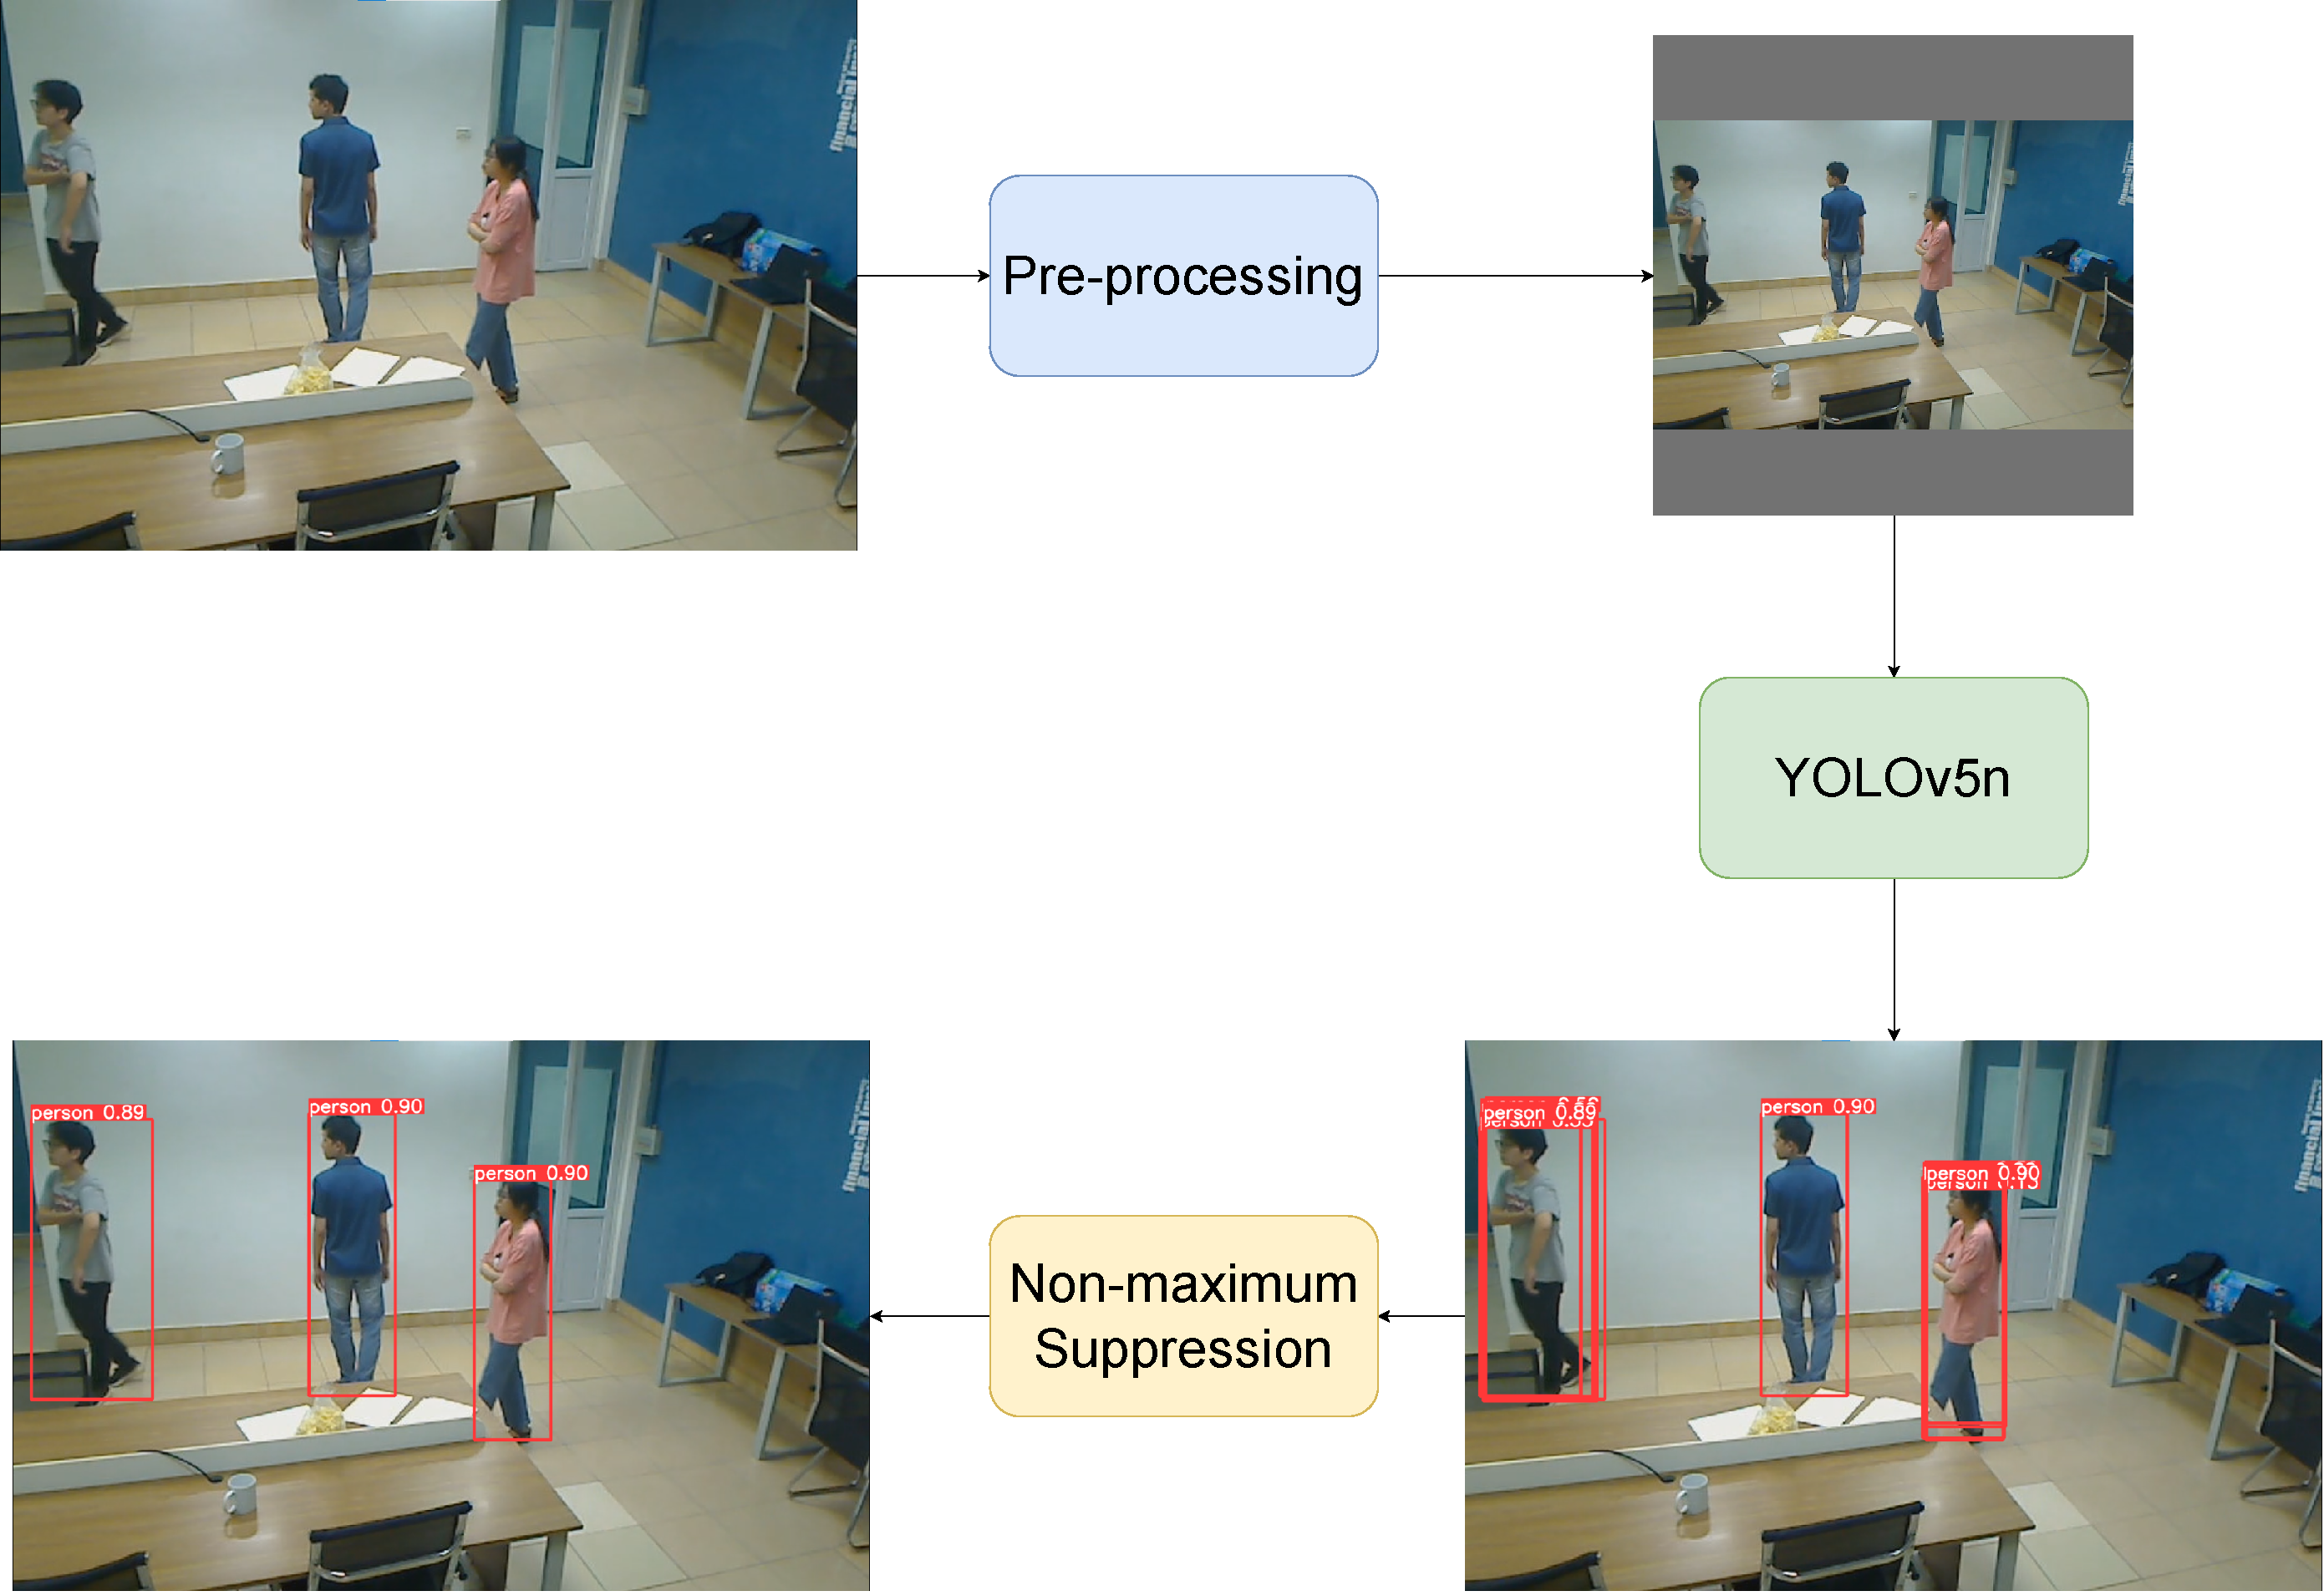
\includegraphics[width=\linewidth]{Figure/object_detection.pdf}
\caption{The process of human detection.}
\label{fig:detect_result}
\end{figure}

The human detection model takes input frames and detects humans on them. Figure~\ref{fig:detect_result} illustrates three parts of the human detection process. Before feeding inputs into the human detection model, they are first pre-processed. After obtaining bounding boxes from the model, they will be processed by the non-maximum suppression algorithm to get the final outputs.

Each output bounding box will have the following components:
\begin{outline}
 \1 Coordinates of the box in the current frame. The coordinates contain four elements: $xmin$, $ymin$, $xmax$, and $ymax$.
    \2 $xmin$ is the left bound of the box.
    \2 $ymin$ is the upper bound of the box.
    \2 $xmax$ is the right bound of the box.
    \2 $ymax$ is the lower bound of the box.
 \1 The class of the box. In this case, this element is trivial because there is only one class in the detection model.
 \1 The confidence score. This indicator shows us how confident the model is in the prediction. The confidence score ranges from 0 to 1. The higher the confidence score, the more confident the model is in the prediction.
\end{outline}

Outputs from the detection model are utilized by the feature extraction model and the tracking algorithm. YOLOv5n, the nano version of YOLOv5, is used as the object detection model because of its lightweight and low latency characteristics as mentioned in Section~\ref{sec:objdect}. I use the pre-trained weights of YOLOv5n, which has already been trained with the COCO dataset~\cite{lin2014microsoft}. I choose to use this pre-trained instead of training from scratch because this huge dataset has already contained the $person$ class which is the objective class of the desired model.

\subsubsection{Pre-processing}
Before feeding images into the detection model, they need to be pre-processed to transform all images of different resolutions into the same format. The pre-processing method must be exactly the same as during model training. The desired size is $384\times384$ and raw images are resized to this resolution. I choose this resolution instead of the original resolution $640\times640$ of YOLOv5n to reduce the computing cost and reduce latency. Computing on the original resolution is a burden for the edge device.

First of all, the larger dimension of the raw image is resized to $384$ and the other dimension is resized with the same ratio. This makes the length of the second dimension to be lower or equal to $384$. Therefore, to achieve the desired length of 384, both sides of the second dimension are padded equally with gray color of value $(114, 114, 114)$. Moreover, all the pixel values are divided by $255$ to normalize the image to the range $[0, 1]$.

% \begin{figure}[h!]
% \centering
% \includegraphics[width=\linewidth]{Figure/preprocess.pdf}
% \caption{The result of the pre-processing process of the human detection model.}
% \label{fig:preprocess}
% \end{figure}

\subsubsection{Detecting with YOLOv5n}
As mentioned before, the pre-trained weights of YOLOv5n were used. These weights have been pre-trained with the COCO dataset~\cite{lin2014microsoft}. I only use the $person$ class and ignore all other classes. This version of pre-trained weights was trained with the input size of $640\times640$. Although this input size is not my desired size which is $384\times384$, this pre-trained model can still be utilized well because of the pyramid architecture of YOLOv5n which enable it to be robust with objects of different size. Moreover, input images of arbitrary resolutions can also be computed because of the CNN architecture. Due to limited computing resources on edge devices, I choose to infer the model on a smaller resolution to lower the computation cost. Moreover, this model is further converted into a TensorRT engine for high-performance deep learning inference on Jetson Nano. Its weights are quantized from 32-bit floating points to 16-bit floating points for a faster computation speed.

After feeding the processed input into the model, many detected bounding boxes overlap with each other. Therefore, a post-processing algorithm is needed to remove redundant bounding boxes and it is called Non-maximum suppression which will be presented in the next part.

% \begin{figure}[h!]
% \centering
% \includegraphics[width=0.8\linewidth]{Figure/detect_overlap.png}
% \caption{The raw results of human detection model.}
% \label{fig:detect_overlap}
% \end{figure}

\subsubsection{Non-maximum suppression}
The detection model produces a lot of overlapping detections. A single individual in the image can have more than one bounding box. One object with multiple corresponding bounding boxes can cause trouble at a later stage. All unnecessary bounding boxes need to be filtered out and only one bounding box is remained. This remaining bounding box is chosen by the non-maximum suppression algorithm. NMS helps to take one best bounding box out of many overlapping bounding boxes. It chooses a pair of overlapping bounding boxes by IoU threshold which is described in Section~\ref{metric:iou} and removes the one with a lower confidence score as shown in Figure~\ref{fig:nms_score}. The process is repeated until there is no pair of overlapping detections left. Through experiments, the IoU score was chosen to be $0.45$ because this threshold showed the best result. An excessively high threshold may cause unnecessary bounding boxes to persist, whereas an excessively low threshold may lead to the merging of bounding boxes belonging to two different individuals who are standing next to each other. Besides, before running NMS, all bounding boxes that have a confidence score lower than $0.45$ are first filtered out to reduce the workload for NMS.

\begin{figure}[h!]
\centering
\includegraphics[width=0.8\linewidth]{Figure/nms_score.pdf}
\caption{NMS filters out the bounding box with the lower confidence score in a candidate pair of overlapping bounding boxes.}
\label{fig:nms_score}
\end{figure}

After running NMS, we obtain bounding boxes with no high overlapping. These final bounding boxes are utilized in later parts: Human feature extraction in Section~\ref{subsec:hfext} and Human tracking in Section~\ref{subsec:hutrack}.

\subsection{Human feature extraction}
\label{subsec:hfext}
Feature extraction model plays a crucial role in the human monitoring system. It provides the system with the ability to Re-ID across different cameras. Moreover, it also improves the quality of the tracking algorithm within independent cameras. The human feature extraction model takes the pre-processed ROI cut from the raw image based on the detected human bounding box as input and it outputs a 224-dimensional feature vector as shown in Figure~\ref{fig:feature}. These feature vectors are sent to the server to store and conduct cross-camera re-identification. The server assesses whether the vectors received from various edge devices belong to the same individual or not. In addition, these features are also used by the human tracking algorithm in Section~\ref{subsec:hutrack}.

\begin{figure}[h!]
\centering
\includegraphics[width=\linewidth]{Figure/overview_feature.pdf}
\caption{The process of human feature extraction.}
\label{fig:feature}
\end{figure}

This thesis proposes a customized version of MobileNetV2 as the backbone of the feature extraction model to create a lightweight architecture suitable for edge devices with limited resources. Since the computation time of the human feature extraction model increases with the number of people in the frame, this model needs to be very lightweight. Therefore, I use a customized version of the original MobileNetV2 architecture to further reduce latency.

The proposed model is trained on public datasets and subsequently deployed on edge devices. Furthermore, this model is also converted to TensorRT format as the object detection model for high-performance inference on Jetson Nano. Despite this, the trained weights still use 32-bit floating points to maintain the accuracy of the model. This is necessary because the output features vector needs to be accurate in order to accurately match individuals across multiple cameras.

\subsubsection{Pre-processing}
\label{subsubsec:deep_preprocess}
Before feeding the images into the model, they need to be pre-processed to bring images of different resolutions to the desired size $192\times64$. First of all, the width of the input image is resized to $64$, and the height of the image is resized correspondingly with the same ratio. Next, if the height of the resized image is larger or equal to $192$, this dimension will be resized to shrink it to $192$. Conversely, if the height of the resized image is less than $192$, black pixels with a value of $0$ will be added to the bottom of the image until the height is $192$. Moreover, the pixel values of the pre-processed image are then divided by $255$ to map the value range to $[0, 1]$.

% \begin{figure}[h!]
% \centering
% \includegraphics[width=0.5\linewidth]{Figure/deep_preprocess.pdf}
% \caption{The result of the pre-processing process of the human feature extraction model.}
% \label{fig:deep_preprocess}
% \end{figure}

\subsubsection{Tailored MobileNetV2 as backbone}
Original MobileNetV2 is tailored to further reduce the number of parameters. Instead of using the original MobileNetV2, a tailored model which only contains a portion of MobileNetV2 as the backbone is used. The top of the original MobileNetV2 is removed and the output is taken from block $12^{th}$. Next, a global max pooling layer is applied to shrink the tensor into a vector. Moreover, this layer is followed by a batch normalization layer and a 0.2-dropout layer respectively. The dropout layer is added to deal with the overfitting problem. Finally, a 224-dimensional fully connected dense layer is added to be the output of this model. This tailored human feature extraction model has a total of $0.6$ millions parameters. This lightweight architecture enables this model to be implemented on edge devices.

\subsubsection{Distance function}
With each image fed into the model, one representative feature vector is desired to be obtained. However, not every detection has a corresponding vector. Only detections with a height-over-width ratio smaller than $10$ and greater than $0.9$ have their embeddings. This rule was set to avoid extracting features for bounding boxes of occluded people or wrong detections because utilizing these bad detections worsens the performance of the module. The similarity between two human images is determined by comparing the corresponding feature vectors using a distance function. Specifically, the distance function is a slight modification of the cosine similarity function which is described in Equation~\ref{eq:dist_func}. This distance ranges from $0$ to $1$. The smaller the distance is, the more similar the pair of vectors is.

\begin{equation}\label{eq:dist_func}
    f(A, B) =  \dfrac {1 - g(A, B)} {2}
\end{equation}

\begin{equation}\label{eq:cosine}
    g(A, B) = \dfrac {A \cdot B} {\left\| A\right\| _{2}\left\| B\right\| _{2}}
\end{equation}
In which:
\begin{outline}
 \1 $f$ is the desired distance function, $g$ is the cosine similarity function.
 \1 The numerator in the cosine similarity function is the dot product of two vectors $A$ and $B$.
 \1 $\left\| A\right\| _{2}$ is the L2 norm of vector A.
 \1 $\left\| B\right\| _{2}$ is the L2 norm of vector B.
\end{outline}

\subsection{Human tracking}
\label{subsec:hutrack}

\begin{figure}[h!]
\centering
\includegraphics[width=\linewidth]{Figure/track_flow.pdf}
\caption{Overview of the tracking algorithm.}
\label{fig:track}
\end{figure}

The human tracking algorithm helps to track individuals moving in the frames, it helps to remain the same identity for a person moving in a camera. Figure~\ref{fig:track} demonstrates the function of the tracking algorithm, it remains the identity for each person moving in a camera. The tracking algorithm takes bounding boxes from the detection model in Section~\ref{subsec:hudect} and tracked objects from the previous frame as input. Moreover, the feature of each bounding box is extracted by the extraction model in Section~\ref{subsec:hfext} to additionally provide visual information for the tracking algorithm. The outputs of this algorithm are tracked entities throughout the input stream. Each entity has a unique identification number, and people from different frames with the same identification number are the same person. The information about tracked humans including the identification number, coordinates of the bounding box, and extracted feature are sent to the server. Then, this information can help the system to match an entity from one camera to another camera and collect the statistics of people entering the room.

\subsubsection{Association cost function}
First of all, I introduce three association cost functions which are used in the next part, Data association, where all the tracking works happen. These functions calculate the cost between tracked objects and detected bounding boxes produced by the detection model or between two lists of tracked objects. The lower the cost is, the higher probability that the detected bounding box and the tracked object, or two tracked objects are matched. The first association cost function is described in Equation~\ref{eq:cost1}.

\begin{equation}\label{eq:cost1}
    c_{1}(A, B) = 1 - \dfrac {A \cap B} {A \cup B}
\end{equation}
In which:
\begin{outline}
 \1 $A$ and $B$ are detected bounding boxes or estimated bounding boxes of tracked objects using the Kalman filter~\cite{kalman}.
 \1 $A \cap B$ is the intersection area of two bounding boxes.
 \1 $A \cup B$ is the union area of two bounding boxes.
\end{outline}

The second and the third association cost functions are defined as follows:

\begin{equation}\label{eq:cost2}
    c_{2}(A, B) = f(M(A), M(B))
\end{equation}

\begin{equation}\label{eq:cost3}
    c_{3}(A, B) = \lambda\times c_{1}(A, B) + (1-\lambda)\times c_{2}(A, B)
\end{equation}
In which:
\begin{outline}
 \1 $A$ and $B$ are detected bounding boxes or estimated bounding boxes of tracked objects using the Kalman filter~\cite{kalman}.
 \1 $c_{1}$ is defined in Equation~\ref{eq:cost1} as the first association cost function.
 \1 $f$ is defined in Equation~\ref{eq:dist_func} as the visual distance function.
 \1 $M$ represents the function that maps from ROI to the embedding vector by feeding the ROI into the human feature extraction model. However, in this case, if $X$ is a tracked object, $M(X)$ refers to extracted feature vector of detection from the previous frame of the tracked object $X$.
 \1 $\lambda$ is a weight factor. In this case, $0.3$ is chosen to be the value of $\lambda$.
\end{outline}

\subsubsection{Data association}
\label{subsec:dataasso}

Data association is the main component in charge of tracking objects. It helps to assign detections or newly initialized tracked objects with existing tracked objects. This algorithm takes two lists $A$ and $B$ as input: one list of tracked entities and one list of detections or two lists of tracked entities. Then, it creates a cost matrix of these two lists based on an association cost function and optimally assign each bounding box or newly initialized tracked object with each tracked target by the Hungarian algorithm. Moreover, there is also a threshold to prevent assignments where detection is too different from the estimation of a tracked object.

Before going into steps to track humans, I first introduce two states of a tracked object. Each tracked objects have an important attribute called $hit\_counter$. The first state of a tracked object is called $alive$ state, it is the state where $hit\_counter$ is greater than $0$. If a tracked object is matched with a bounding box, its $hit\_counter$ will increase. Moreover, $hit\_counter$ decreases when the corresponding tracked object doesn't have any match. If $hit\_counter$ is higher than a predefined threshold, that tracked object will be officially initialized. It helps the algorithm to be robust against false detections. On the other hand, if the $hit\_counter$ drops below $0$, the tracked object moves to the $dead$ state. In this state, the life cycle of a tracked object does not immediately end. A tracked object will only be completely removed if it is in the $dead$ state and does not have any match in several consecutive frames. Otherwise, if a $dead$ tracked object is matched, the $hit\_counter$ will increase above $0$ and this tracked object is moved back to the $alive$ state.

Next, four main steps of tracking are discussed, these four main steps are executed in every frame. In the first step, $A$ contains initialized $alive$ tracked objects, and $B$ contains new detections. The association cost function is $c_3$ in Equation~\ref{eq:cost3} with a threshold of $0.6$. In this step, if either $c_1$ in Equation~\ref{eq:cost1} is greater than $0.98$ or one of the bounding boxes of $A$ or $B$ does not have a feature embedding, then the cost will be set to $1$. This step uses the cost function utilized from both geometry and visual features which may improve the tracking performance in occlusion scenarios. However, if bounding boxes are too different from each other or any bounding box does not have an embedding feature, they can not be matched.

In the second step, $A$ contains unmatched initialized $alive$ tracked objects from step one. $B$ consists of unmatched detections from step one. The cost function is $c_1$ in Equation~\ref{eq:cost1} with a threshold of $0.7$. This step only considers the coordinates of bounding boxes to calculate the cost.

Next, in the third step, $A$ contains uninitialized $alive$ tracked objects and $B$ contains unmatched detections from the second step. The association cost function is $c_1$ in Equation~\ref{eq:cost1} with a threshold of $0.7$. This step also only considers the coordinates of bounding boxes to calculate the cost.

In the final step, $A$ is the combination of unmatched initialized $alive$ tracked objects from step two and $dead$ tracked objects. $B$ consists of matched uninitialized $alive$ tracked objects from step three. The cost function is $c_2$ in Equation~\ref{eq:cost2} with a threshold of $0.2$. This final step is used to match objects that have disappeared from the camera for a short period. In addition, it also improves the performance in occlusion scenarios.

After tracked objects are obtained, information about tracked people including the identification number, coordinates of the bounding box, and extracted feature are sent to the server. Based on received information from multiple cameras, the server can know exactly when an individual enters the room, which room he or she enters, and where he or she goes to in that specific room.

\section{Implementation of hardware}
\label{sec:hardware}

\begin{figure}[h!]
\centering
\includegraphics[width=\linewidth]{Figure/hardware.pdf}
\caption{Demonstration of hardware implementation with red texts are the hardware.}
\label{fig:hardware}
\end{figure}

This section focuses on the usage of hardware for this thesis, the reason to choose them, and their specifications including computing edge devices, Jetson Nano, webcams, and other peripheral devices. The utilization of hardware is shown in Figure~\ref{fig:hardware}.

\subsection{NVIDIA Jetson Nano developer kit}
\label{subsec:jetsonnano}
NVIDIA Jetson Nano developer kit~\cite{jetsonnano} is a small, compact single-board computer developed for AI applications. It enables applications to run multiple neural networks in parallel. It is suitable for embedded systems, robots that require high-performance inference. Jetson Nano was chosen instead of Raspberry Pi 4~\cite{raspberry} because it has stronger computing power. An edge device with too low computing power does not have the capability to run many deep learning models on a single board even when models have been tailored to be lighter. The detailed technical specifications of Jetson Nano can be seen in Table~\ref{table:jetson}. Jetson Nano can run with a minimum power consumption of only 5 watts and a maximum of up to 10 watts.

\begin{table}[h!]
\centering
\begin{tabular}{||l | l ||} 
\hline 
CPU & Quad-core ARM A57 @ 1.43 GHz \\
\hline
GPU & 128-core Maxwell \\
\hline
Memory & 4 GB 64-bit LPDDR4 25.6 GB/s \\ 
\hline
USB & 4x USB 3.0, USB 2.0 Micro-B \\ 
\hline
Display & HDMI and display port \\ 
\hline
\end{tabular}
\caption{Technical specifications of NVIDIA Jetson Nano Developer Kit.}
\label{table:jetson}
\end{table}

\subsection{Webcams}
This thesis uses three types of USB webcams: Logitech C270 HD, Logitech HD B525, and Logitech HD C905. They are connected to the Jetson Nano via a USB port. All of them have a video resolution of 720p. Each Jetson Nano has one webcam.

\subsection{Other devices}
Jetson Nano is also connected to other peripherals such as the JM101 fingerprint sensor, environment sensors like the DHT11 temperature and humidity sensor, and the MQ135 air quality sensor. However, the development of applications using these devices is carried out by other members of the research team and is beyond the scope of this thesis. These devices can be seen in Figure~\ref{fig:finger} and Figure~\ref{fig:sensor}.

\begin{figure}[h!]
\centering
\includegraphics[width=0.6\linewidth]{Figure/finger.jpg}
\caption{Fingerprint sensor JM101.}
\label{fig:finger}
\end{figure}

\begin{figure}[h!]
\centering
\includegraphics[width=0.8\linewidth]{Figure/sensor.jpg}
\caption{Temperature, humidity sensor DHT11 (blue rectangle) and air quality sensor MQ135 (round head).}
\label{fig:sensor}
\end{figure}

\section{Utilization of frameworks}
This section focuses on the utilization of frameworks for this thesis which is shown in Figure~\ref{fig:framework}.

\begin{figure}[h!]
\centering
\includegraphics[width=0.9\linewidth]{Figure/framework.pdf}
\caption{Demonstration of frameworks utilization with red texts are the frameworks.}
\label{fig:framework}
\end{figure}

\subsection{Tensorflow and Pytorch}
TensorFlow~\cite{tensorflow} and PyTorch~\cite{pytorch} are used to develop the human detection model and human feature extraction model of this thesis. Both of the models are later converted to TensorRT format for efficient inference on Jetson Nano. They are two of the most widely used open-source machine learning, deep learning frameworks. They are used by a large number of engineers, scientists all over the world to develop AI models and applications.

\subsection{TensorRT}
\label{subsec:tensorrt}
TensorRT~\cite{tensorrt} is a library designed for high-performance deep learning inference that contains an optimizer and runtime for deep learning inference. It enables AI applications to achieve low latency and high throughput. TensorRT can optimize models to run especially well on NVIDIA GPUs. Therefore, TensorRT is used to optimize the human detection model and the human feature extraction model of this thesis to run on Jetson Nano. TensorRT uses post-quantization to increase the inference speed of the human detection model by converting its weights from 32-bit to 16-bit floating points. On the other hand, the feature extraction model is already lightweight, and therefore its weights are kept as 32-bit floating points to maintain the performance of the model.

\subsection{OpenCV}
OpenCV~\cite{opencv} is an open-source image processing and computer vision library. OpenCV was chosen to be used because it provides easy-to-use APIs to read frames from connected USB cameras. Moreover, OpenCV also provides many useful image-processing APIs. It was used in the pre-processing and post-processing parts of the human detection and human feature extraction model.

\subsection{Norfair}
Norfair~\cite{norfair} is a customizable lightweight Python library for real-time multi-object tracking. Norfair brings convenience when you want to modify a tracking algorithm according to your preferences. Norfair makes it extremely convenient to integrate your own detection model or cost function into the tracking algorithm. Norfair was used to develop the tracking algorithm in this thesis. It helps to integrate the human detection model, the feature extraction model, and the customized cost function into the tracking algorithm easily.

This chapter has presented the flow of the AI module and details about each component in this module. Each component has been carefully researched and customized to solve the raised problem and achieve the objectives of this thesis. Evaluations and deployment results are discussed in the next chapter, Chapter~\ref{chapter:experiment}.
\end{document}